\documentclass{article}[12pt]
\usepackage{graphicx} % Required for inserting images
\usepackage{listings}
\usepackage{hyperref}
\usepackage{tabularx}
\usepackage{float}
\usepackage{subfig}
\usepackage[a4paper, left=1cm, right=1cm]{geometry}

\title{EARIN Lab 5 Report}
\author{Krzysztof Rudnicki, 307585 \\ Jakub Kliszko, 303866  }
\date{\today}

\begin{document}

\maketitle

\section{Exercise Variant 2}
Use \href{https://pytorch.org/vision/stable/generated/torchvision.datasets.MNIST.html#torchvision.datasets.MNIST}{MIST} dataset. Evaluate at least 3 different numbers/values/types of:
\begin{itemize}
    \item learning rate
    \item mini-batch size (including batch containing only 1 example)
    \item number of hidden layers (including 0 hidden layers - linear model)
    \item width (number of neurons in hidden layers)
    \item optimizer type (e.g., SGD, SGD with momentum, Adam)
\end{itemize}

\section{Implementation}
Program can be ran by installing python, moving to project directory and issuing command:
\begin{lstlisting}[language=bash]
python main.py
\end{lstlisting}
Results will be displayed on three 2d scatter plots. \\ 
Plots Title is filled with parameters used abbreviated for space sake \\ 
Abbreviatons meaning: 
\begin{itemize} 
    \item lr - Learning Rate
    \item bs - Batch Size 
    \item hl - Number of Hidden Layers 
    \item w - Width 
    \item Adam or SGD or SGD\_Momentum - Optimizer type
\end{itemize}
Plot types: 
\begin{itemize}
    \item Loss value for learning step
    \item Train Accuracy for epoch
    \item Validation Accuracy for epoch
\end{itemize}

\begin{figure}[H]
    \caption{Exemplary plot of loss for learning Step \\ lr0.001-bs64-hl1-w128-Adam }
    \includegraphics[width=\textwidth]{testsResults/loss/def.png}
    \centering
    \end{figure}
\begin{figure}[H]
    \caption{Exemplary plot of Validation Accuracy for epoch \\ lr0.001-bs64-hl1-w128-Adam }
    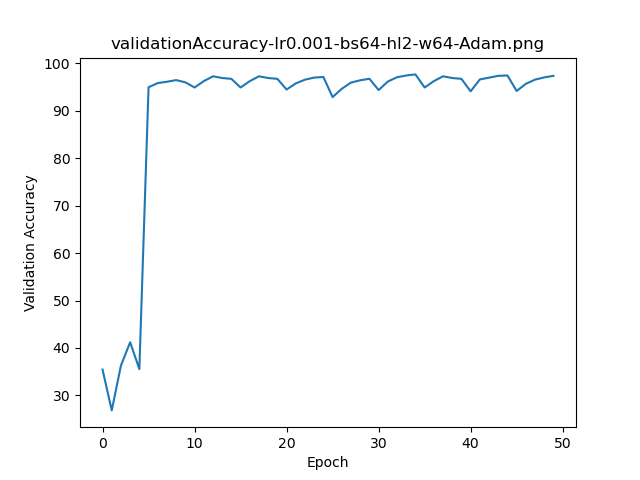
\includegraphics[width=\textwidth]{testsResults/validationAccuracy/validationAccuracy-lr0.001-bs64-hl2-w64-Adam.png}
    \centering
    \end{figure}
\begin{figure}[H]
\caption{Exemplary plot of Train Accuracy for epoch \\ lr0.001-bs64-hl1-w128-Adam }
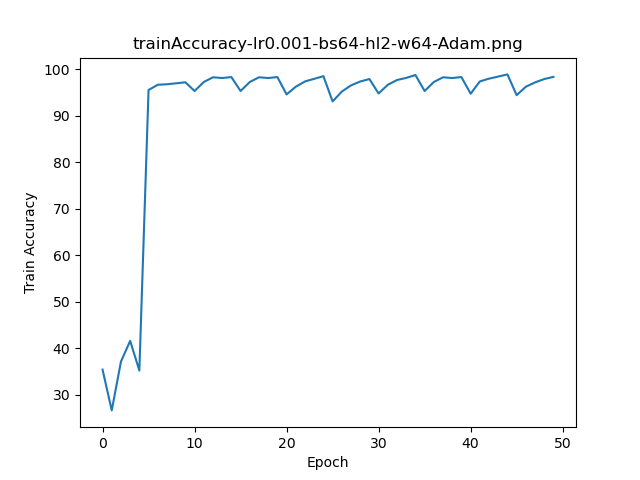
\includegraphics[width=\textwidth]{testsResults/trainAccuracy/trainAccuracy-lr0.001-bs64-hl2-w64-Adam.png}
\centering
\end{figure}
Results will be displayed and saved in the same folder as code directory for further inspection, with file name containing information about input parameters \\
Additionaly speed it took for neural network to run will be saved to results.txt along with what parameters were used \\ 
We decided to run 19 tests in total:
\begin{enumerate} 
    \item learning rate [0.1, 0.01, 0.001] (3 tests)
    \item mini-batch size [1, 64, 128, 256] (4 tests)
    \item number of hidden layers [0, 1, 2, 3] (4 tests)
    \item width [64, 128, 256, 512, 1024] (5 tests)
    \item optimizer type [SGD, SGD\_Momentum, Adam] (3 tests)
\end{enumerate} 
\section{Results}
We have successfully implemented network analyzing MNIST dataset \\ 
\subsection{Loss Graphs}

\subsubsection{Learning Rate}

    \begin{figure}[H]
        \minipage{0.5\textwidth}
        \includegraphics[width=\linewidth]{testsResults/loss/lr/def.png}
        \caption{Default settings + learning rate = 0.001}
        \endminipage\hfill
        \minipage{0.5\textwidth}
        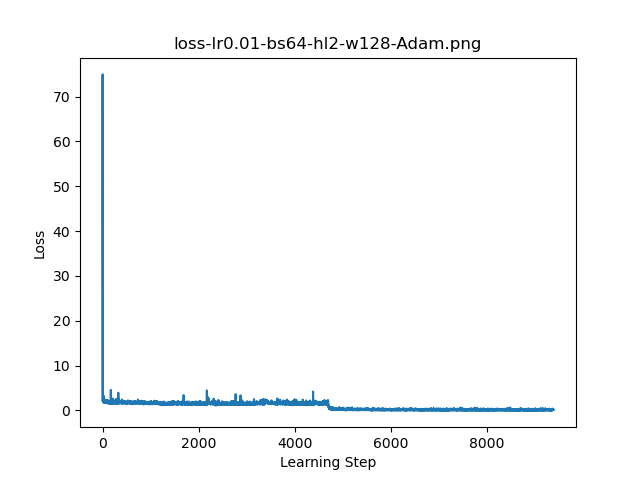
\includegraphics[width=\linewidth]{testsResults/loss/lr/loss-lr0.01-bs64-hl2-w128-Adam.png}
        \caption{Default settings + learning rate = 0.01}
        \endminipage
    \end{figure}
        \begin{figure}[H]
        \minipage{0.5\textwidth}%
        \includegraphics[width=\linewidth]{testsResults/loss/lr/def.png}
        \caption{Default settings + learning rate = 0.1}
        \endminipage
    \end{figure}

\subsubsection{Mini-Batch size}

    \begin{figure}[H]
        \minipage{0.5\textwidth}
        \includegraphics[width=\linewidth]{testsResults/loss/bs/def.png}
        \caption{Default settings + batching size = 64}
        \endminipage\hfill
        \minipage{0.5\textwidth}
        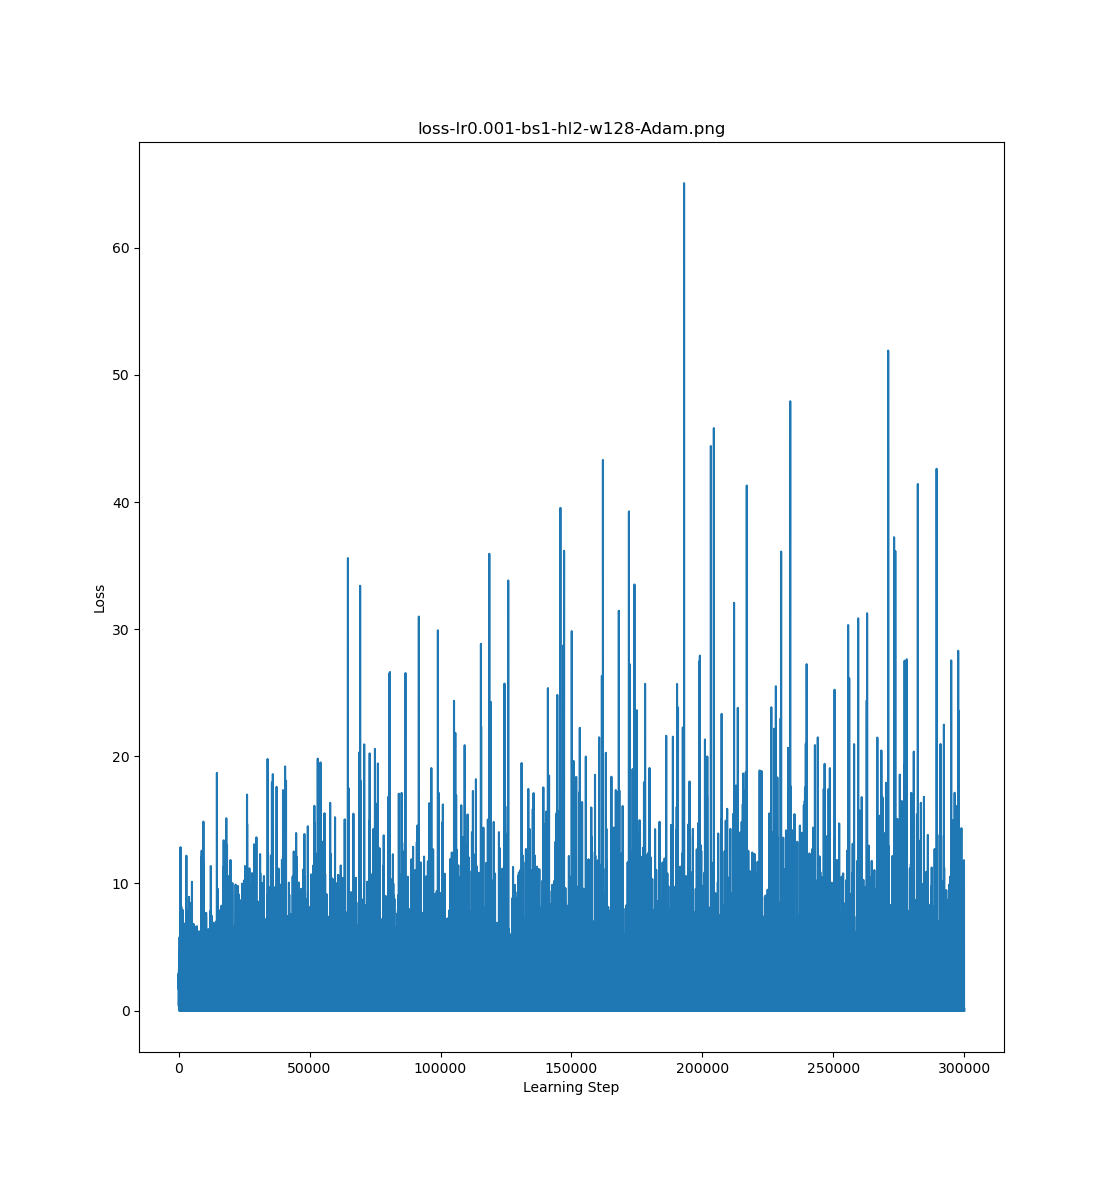
\includegraphics[width=\linewidth]{testsResults/loss/bs/loss-1batch.png}
        \caption{Default settings + batching size = 1}
        \endminipage
    \end{figure}
        \begin{figure}[H]
        \minipage{0.5\textwidth}%
        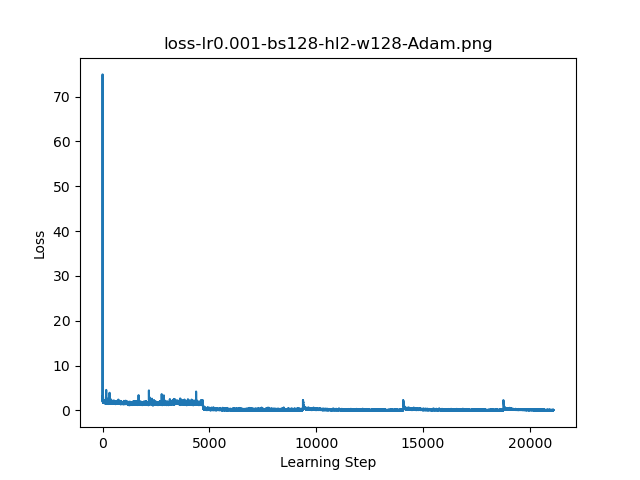
\includegraphics[width=\linewidth]{testsResults/loss/bs/loss-lr0.001-bs128-hl2-w128-Adam.png}
        \caption{Default settings + batching size = 128}
        \endminipage
        \minipage{0.5\textwidth}%
        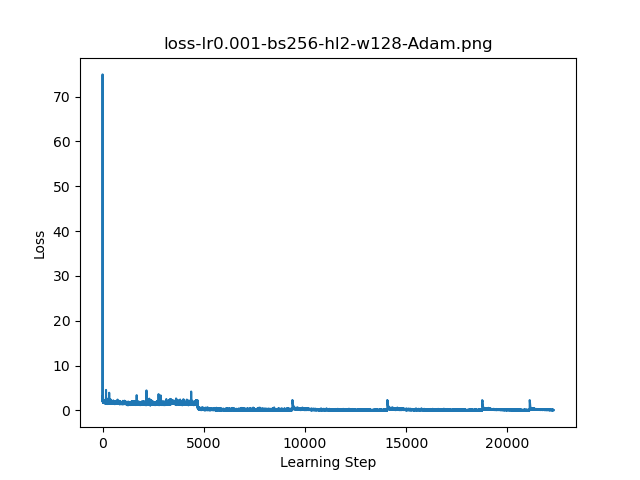
\includegraphics[width=\linewidth]{testsResults/loss/bs/loss-lr0.001-bs256-hl2-w128-Adam.png}
        \caption{Default settings + batching size = 256}
        \endminipage
    \end{figure}

\subsubsection{Number of Hidden Layers}

    \begin{figure}[H]
        \minipage{0.5\textwidth}
        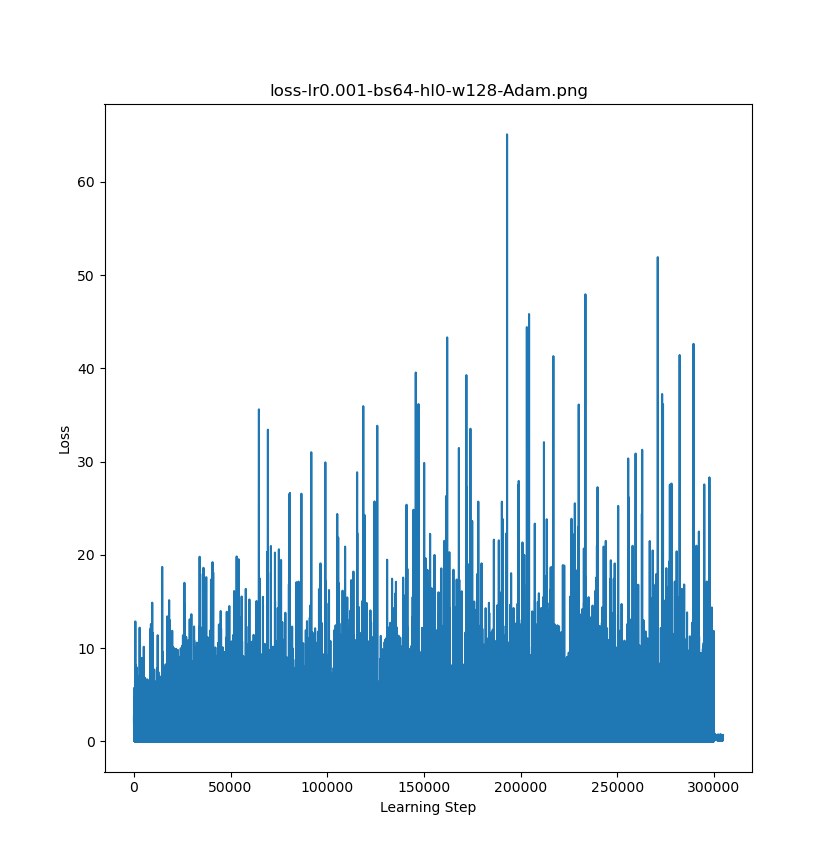
\includegraphics[width=\linewidth]{testsResults/loss/hl/hl0loss.png}
        \caption{Default settings + hidden layers = 0}
        \endminipage\hfill
        \minipage{0.5\textwidth}
        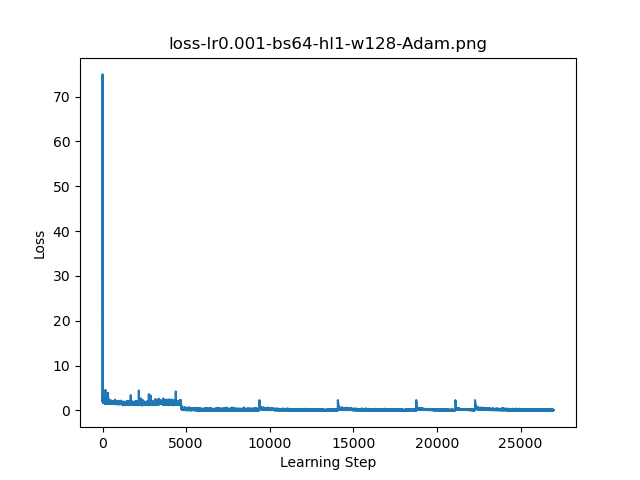
\includegraphics[width=\linewidth]{testsResults/loss/hl/loss-lr0.001-bs64-hl1-w128-Adam.png}
        \caption{Default settings + hidden layers = 1}
        \endminipage
    \end{figure}
        \begin{figure}[H]
        \minipage{0.5\textwidth}%
        \includegraphics[width=\linewidth]{testsResults/loss/hl/def.png}
        \caption{Default settings + hidden layers = 2}
        \endminipage
        \minipage{0.5\textwidth}%
        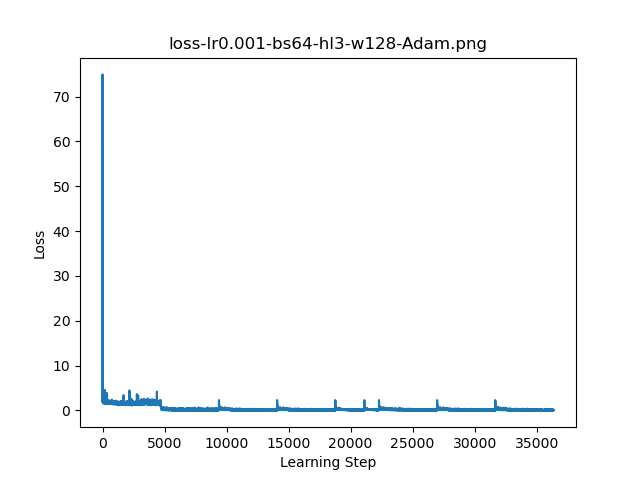
\includegraphics[width=\linewidth]{testsResults/loss/hl/loss-lr0.001-bs64-hl3-w128-Adam.png}
        \caption{Default settings + hidden layers = 3}
        \endminipage
    \end{figure}
    \newpage
\subsubsection{Width}

    \begin{figure}[H]
        \minipage{0.5\textwidth}
        \includegraphics[width=\linewidth]{testsResults/loss/w/def.png}
        \caption{Default settings + width = 128}
        \endminipage\hfill
        \minipage{0.5\textwidth}
        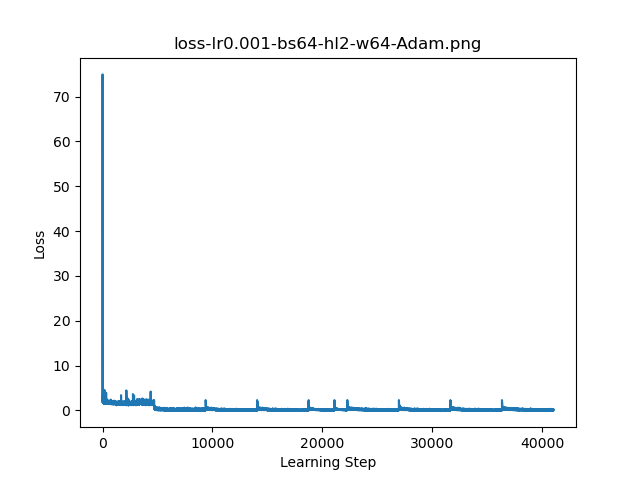
\includegraphics[width=\linewidth]{testsResults/loss/w/loss-lr0.001-bs64-hl2-w64-Adam.png}
        \caption{Default settings + width = 64}
        \endminipage
    \end{figure}
        \begin{figure}[H]
        \minipage{0.5\textwidth}%
        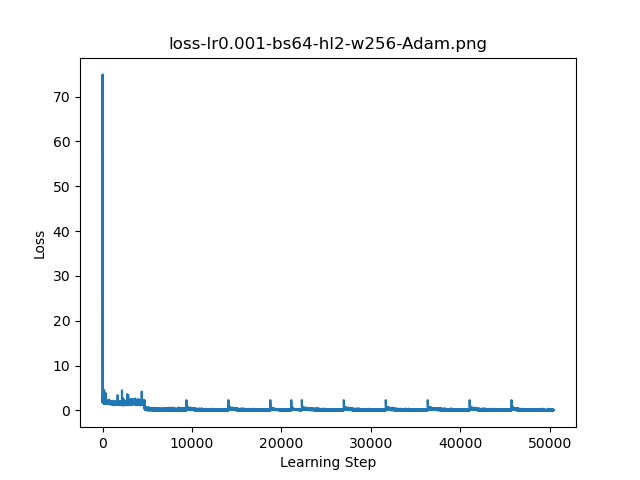
\includegraphics[width=\linewidth]{testsResults/loss/w/loss-lr0.001-bs64-hl2-w256-Adam.png}
        \caption{Default settings + width = 256}
        \endminipage
        \minipage{0.5\textwidth}%
        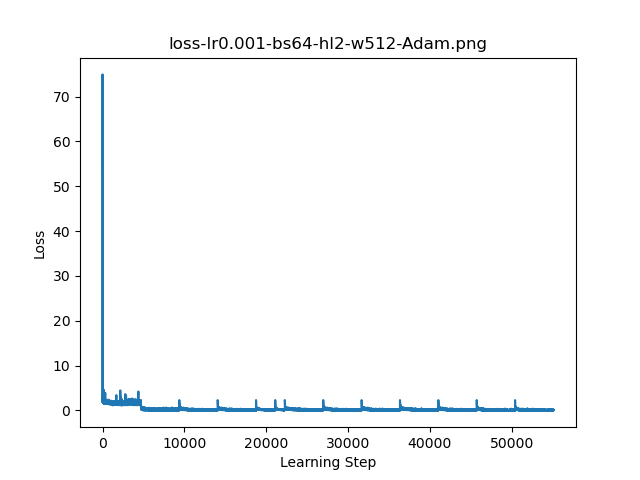
\includegraphics[width=\linewidth]{testsResults/loss/w/loss-lr0.001-bs64-hl2-w512-Adam.png}
        \caption{Default settings + width = 512}
        \endminipage
    \end{figure}
    \begin{figure}[H]
        \minipage{0.5\textwidth}%
        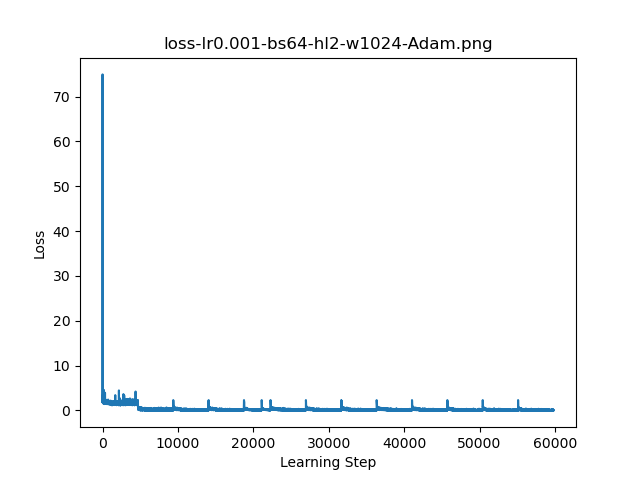
\includegraphics[width=\linewidth]{testsResults/loss/w/loss-lr0.001-bs64-hl2-w1024-Adam.png}
        \caption{Default settings + width = 1024}
        \endminipage
    \end{figure}

\subsubsection{Optimizer Type}

    \begin{figure}[H]
        \minipage{0.5\textwidth}
        \includegraphics[width=\linewidth]{testsResults/loss/optimizer/def.png}
        \caption{Default settings + Adam optimizer}
        \endminipage\hfill
        \minipage{0.5\textwidth}
        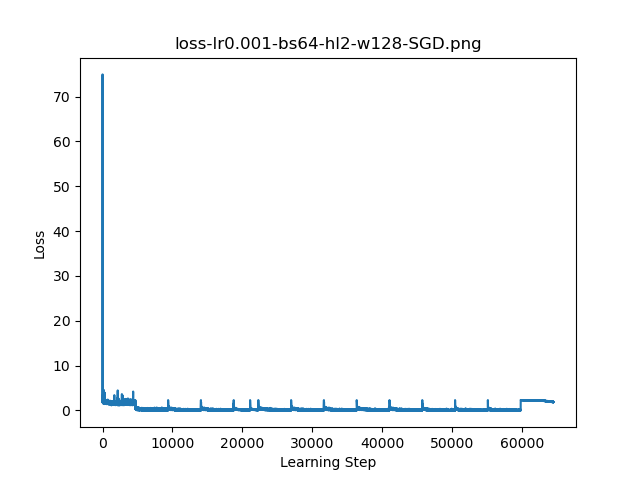
\includegraphics[width=\linewidth]{testsResults/loss/optimizer/loss-lr0.001-bs64-hl2-w128-SGD.png}
        \caption{Default settings + learning rate = 0.01}
        \endminipage
    \end{figure}
        \begin{figure}[H]
        \minipage{0.5\textwidth}%
        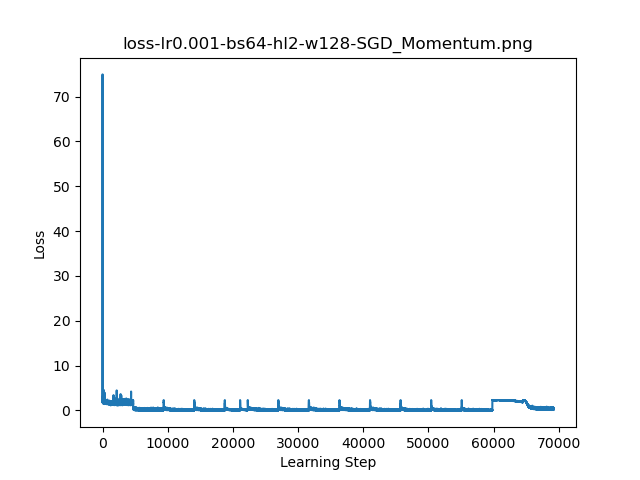
\includegraphics[width=\linewidth]{testsResults/loss/optimizer/loss-lr0.001-bs64-hl2-w128-SGD_Momentum.png}
        \caption{Default settings + SGD\_Momentum optimizer}
        \endminipage
    \end{figure}

\subsection{Train Accuracy Graphs}

\subsubsection{Learning Rate}

    \begin{figure}[H]
        \minipage{0.5\textwidth}
        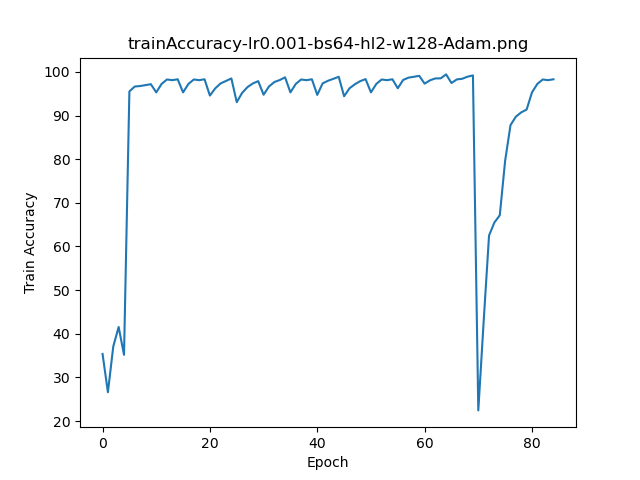
\includegraphics[width=\linewidth]{testsResults/trainAccuracy/def.png}
        \caption{Default settings + learning rate = 0.001}
        \endminipage\hfill
        \minipage{0.5\textwidth}
        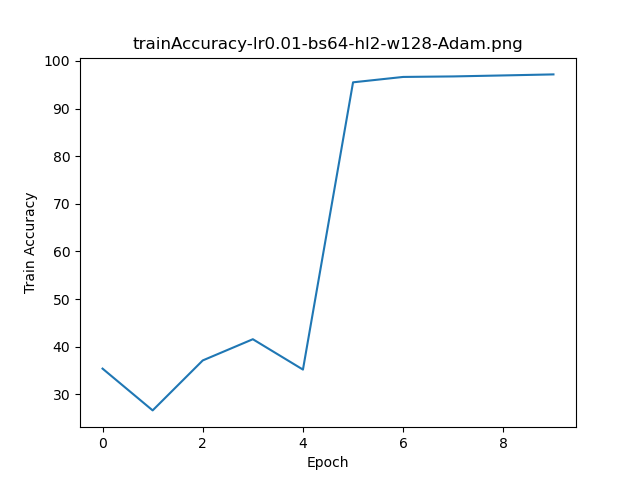
\includegraphics[width=\linewidth]{testsResults/trainAccuracy/trainAccuracy-lr0.01-bs64-hl2-w128-Adam.png}
        \caption{Default settings + learning rate = 0.01}
        \endminipage
    \end{figure}
        \begin{figure}[H]
        \minipage{0.5\textwidth}%
        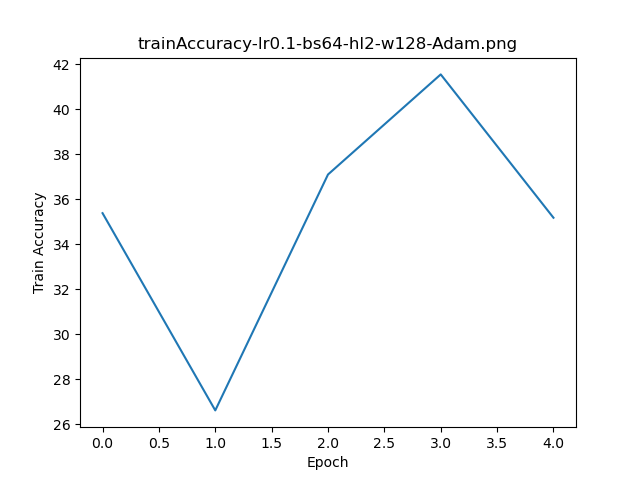
\includegraphics[width=\linewidth]{testsResults/trainAccuracy/trainAccuracy-lr0.1-bs64-hl2-w128-Adam.png}
        \caption{Default settings + learning rate = 0.1}
        \endminipage
    \end{figure}

\subsubsection{Mini-Batch size}

    \begin{figure}[H]
        \minipage{0.5\textwidth}
        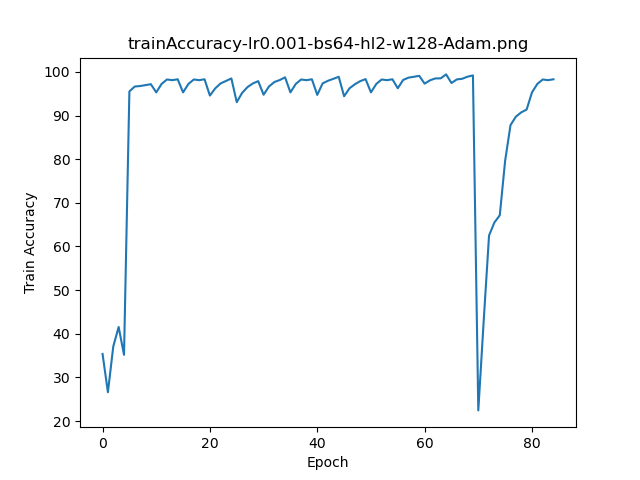
\includegraphics[width=\linewidth]{testsResults/trainAccuracy/def.png}
        \caption{Default settings + batching size = 64}
        \endminipage\hfill
        \minipage{0.5\textwidth}
        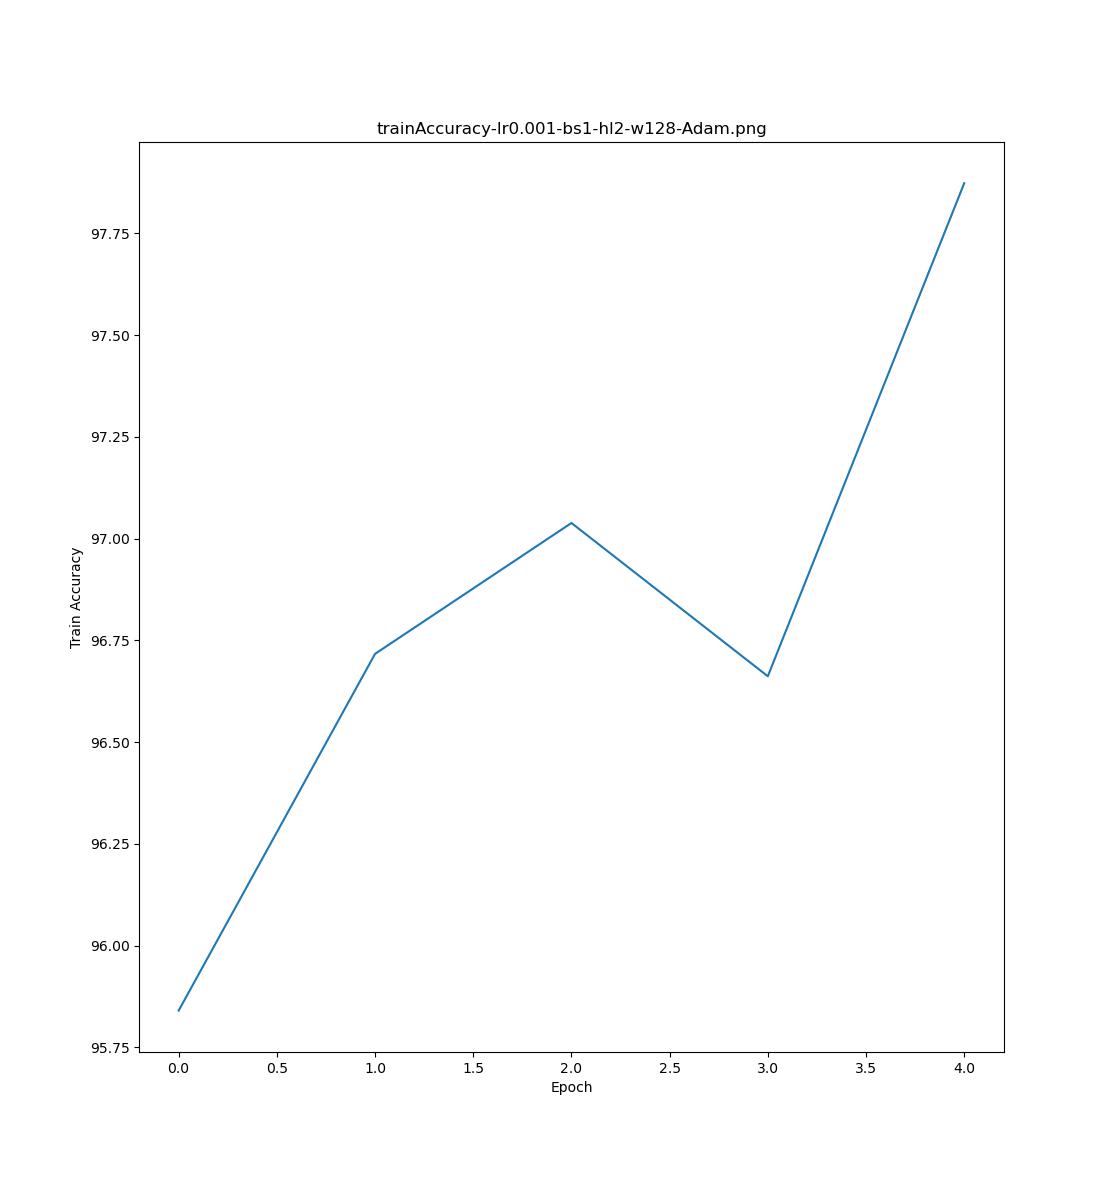
\includegraphics[width=\linewidth]{testsResults/trainAccuracy/trainAccuracy1batch.png}
        \caption{Default settings + batching size = 1}
        \endminipage
    \end{figure}
        \begin{figure}[H]
        \minipage{0.5\textwidth}%
        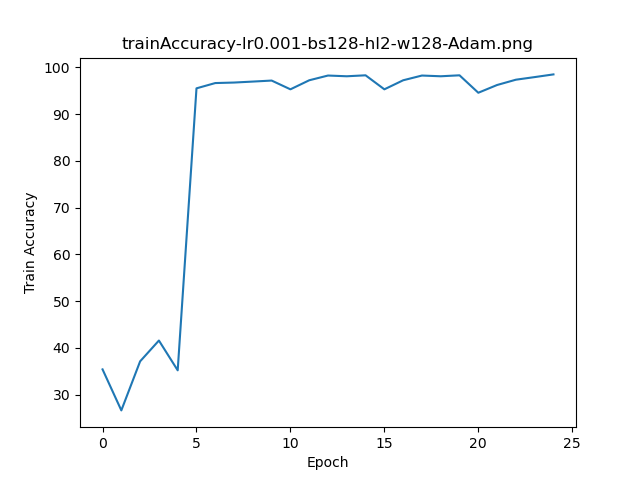
\includegraphics[width=\linewidth]{testsResults/trainAccuracy/trainAccuracy-lr0.001-bs128-hl2-w128-Adam.png}
        \caption{Default settings + batching size = 128}
        \endminipage
        \minipage{0.5\textwidth}%
        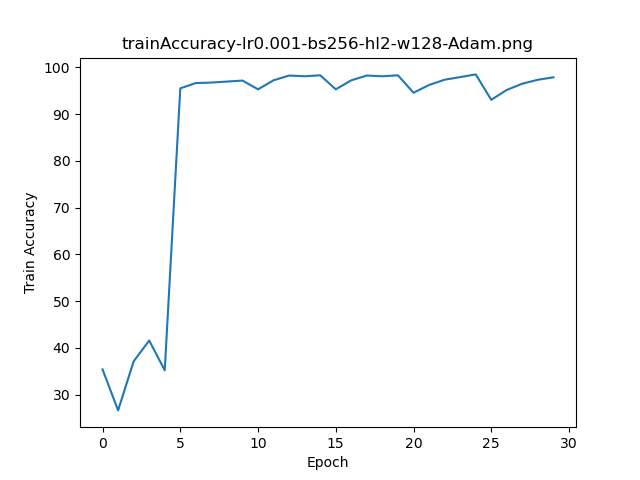
\includegraphics[width=\linewidth]{testsResults/trainAccuracy/trainAccuracy-lr0.001-bs256-hl2-w128-Adam.png}
        \caption{Default settings + batching size = 256}
        \endminipage
    \end{figure}

\subsubsection{Number of Hidden Layers}

    \begin{figure}[H]
        \minipage{0.5\textwidth}
        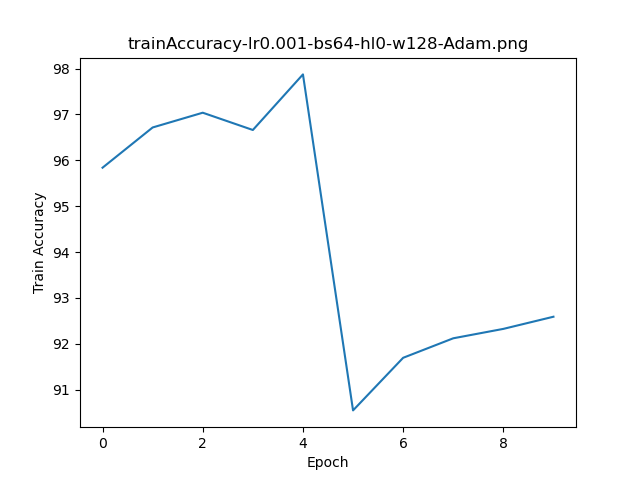
\includegraphics[width=\linewidth]{testsResults/trainAccuracy/trainAccuracy-lr0.001-bs64-hl0-w128-Adam.png}
        \caption{Default settings + hidden layers = 0}
        \endminipage\hfill
        \minipage{0.5\textwidth}
        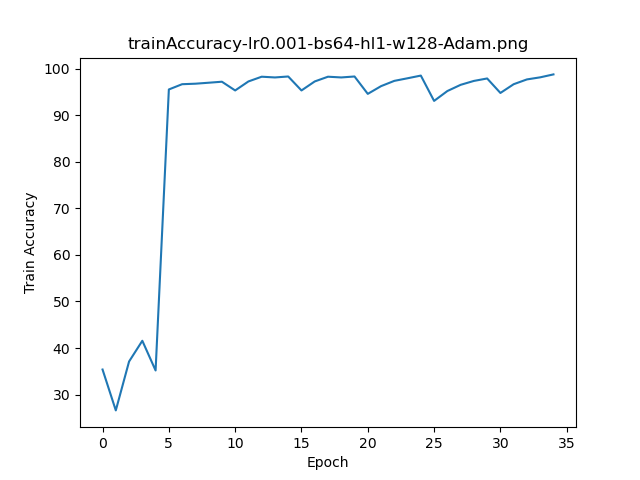
\includegraphics[width=\linewidth]{testsResults/trainAccuracy/trainAccuracy-lr0.001-bs64-hl1-w128-Adam.png}
        \caption{Default settings + hidden layers = 1}
        \endminipage
    \end{figure}
        \begin{figure}[H]
        \minipage{0.5\textwidth}%
        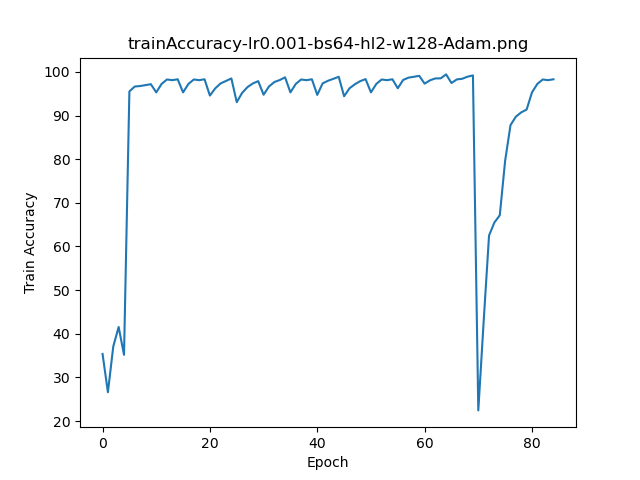
\includegraphics[width=\linewidth]{testsResults/trainAccuracy/def.png}
        \caption{Default settings + hidden layers = 2}
        \endminipage
        \minipage{0.5\textwidth}%
        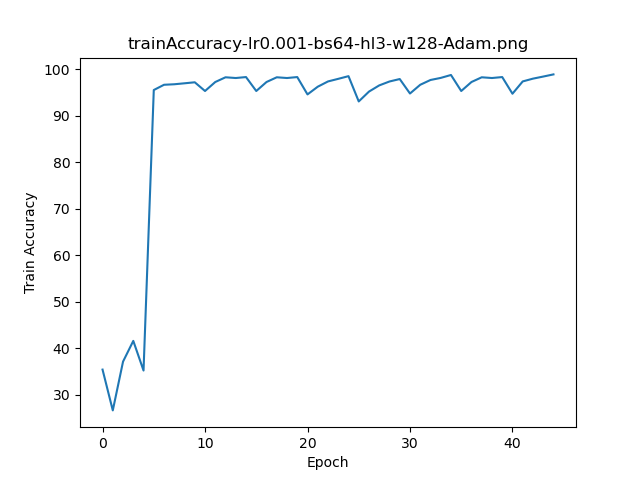
\includegraphics[width=\linewidth]{testsResults/trainAccuracy/trainAccuracy-lr0.001-bs64-hl3-w128-Adam.png}
        \caption{Default settings + hidden layers = 3}
        \endminipage
    \end{figure}

    \newpage
\subsubsection{Width}

    \begin{figure}[H]
        \minipage{0.5\textwidth}
        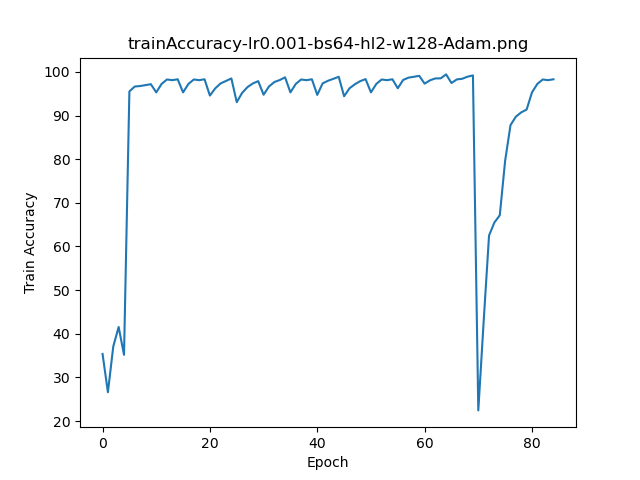
\includegraphics[width=\linewidth]{testsResults/trainAccuracy/def.png}
        \caption{Default settings + width = 128}
        \endminipage\hfill
        \minipage{0.5\textwidth}
        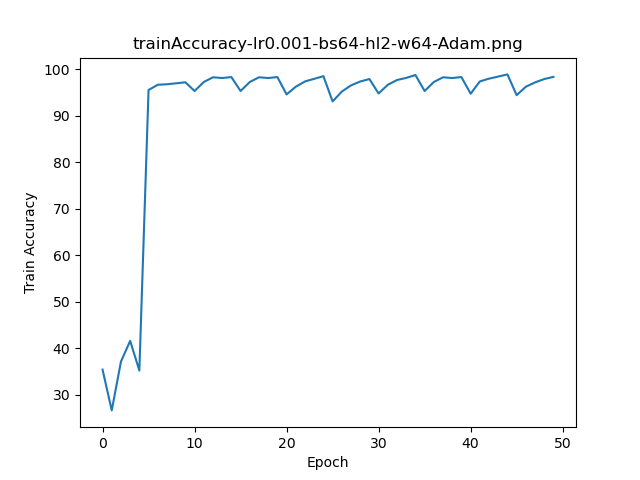
\includegraphics[width=\linewidth]{testsResults/trainAccuracy/trainAccuracy-lr0.001-bs64-hl2-w64-Adam.png}
        \caption{Default settings + width = 64}
        \endminipage
    \end{figure}
        \begin{figure}[H]
        \minipage{0.5\textwidth}%
        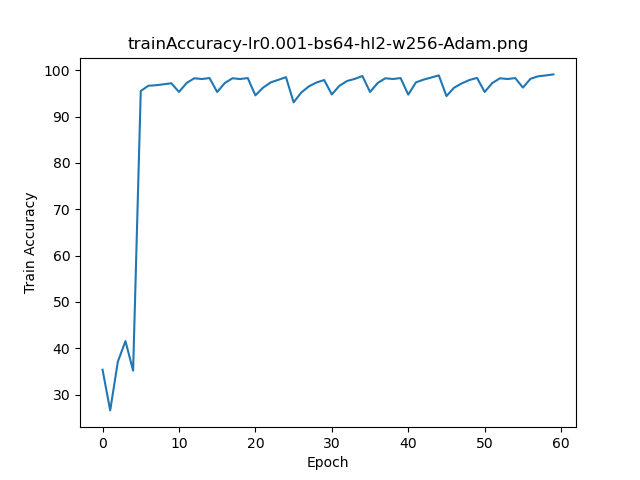
\includegraphics[width=\linewidth]{testsResults/trainAccuracy/trainAccuracy-lr0.001-bs64-hl2-w256-Adam.png}
        \caption{Default settings + width = 256}
        \endminipage
        \minipage{0.5\textwidth}%
        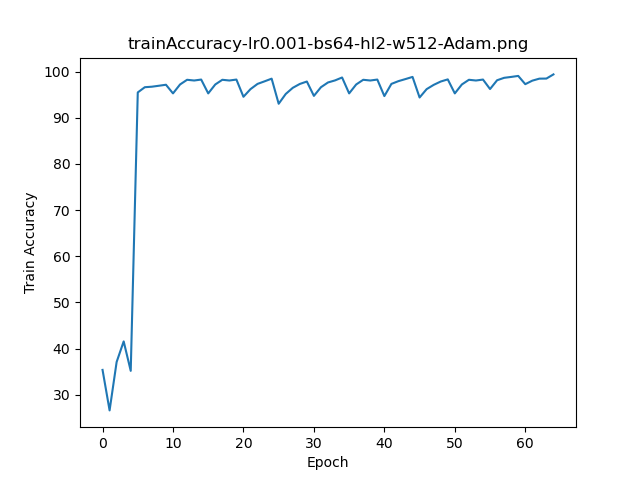
\includegraphics[width=\linewidth]{testsResults/trainAccuracy/trainAccuracy-lr0.001-bs64-hl2-w512-Adam.png}
        \caption{Default settings + width = 512}
        \endminipage
    \end{figure}
    \begin{figure}[H]
        \minipage{0.5\textwidth}%
        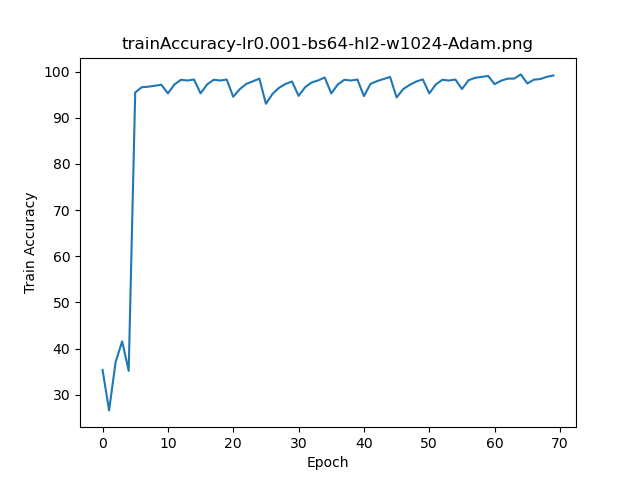
\includegraphics[width=\linewidth]{testsResults/trainAccuracy/trainAccuracy-lr0.001-bs64-hl2-w1024-Adam.png}
        \caption{Default settings + width = 1024}
        \endminipage
    \end{figure}

\subsubsection{Optimizer Type}

    \begin{figure}[H]
        \minipage{0.5\textwidth}
        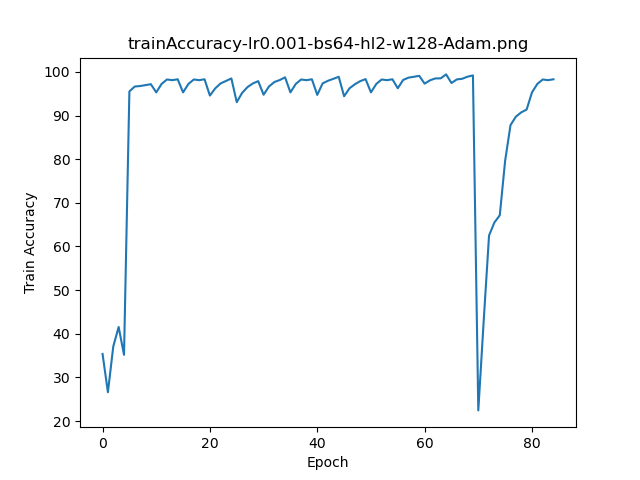
\includegraphics[width=\linewidth]{testsResults/trainAccuracy/def.png}
        \caption{Default settings + Adam optimizer}
        \endminipage\hfill
        \minipage{0.5\textwidth}
        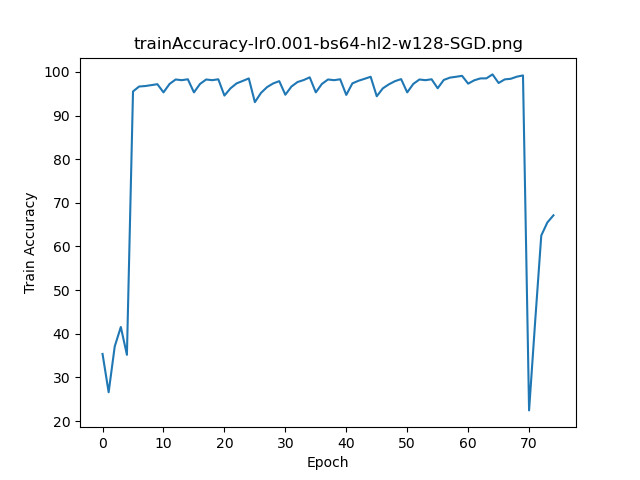
\includegraphics[width=\linewidth]{testsResults/trainAccuracy/trainAccuracy-lr0.001-bs64-hl2-w128-SGD.png}
        \caption{Default settings + learning rate = 0.01}
        \endminipage
    \end{figure}
        \begin{figure}[H]
        \minipage{0.5\textwidth}%
        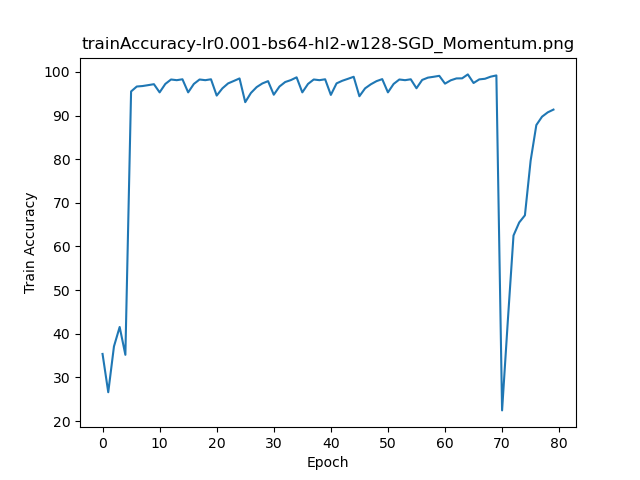
\includegraphics[width=\linewidth]{testsResults/trainAccuracy/trainAccuracy-lr0.001-bs64-hl2-w128-SGD_Momentum.png}
        \caption{Default settings + SGD\_Momentum optimizer}
        \endminipage
    \end{figure}

\subsection{Validation Accuracy Graphs}


\subsubsection{Learning Rate}

    \begin{figure}[H]
        \minipage{0.5\textwidth}
        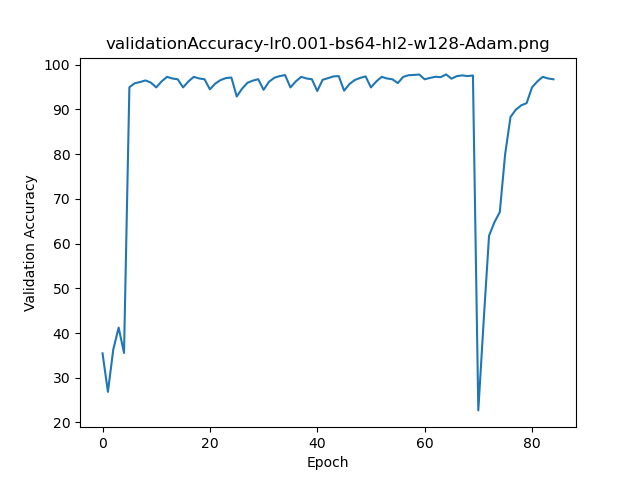
\includegraphics[width=\linewidth]{testsResults/validationAccuracy/def.png}
        \caption{Default settings + learning rate = 0.001}
        \endminipage\hfill
        \minipage{0.5\textwidth}
        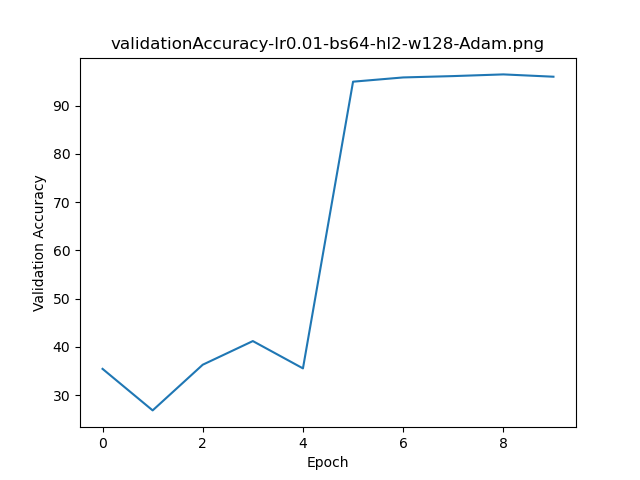
\includegraphics[width=\linewidth]{testsResults/validationAccuracy/validationAccuracy-lr0.01-bs64-hl2-w128-Adam.png}
        \caption{Default settings + learning rate = 0.01}
        \endminipage
    \end{figure}
        \begin{figure}[H]
        \minipage{0.5\textwidth}%
        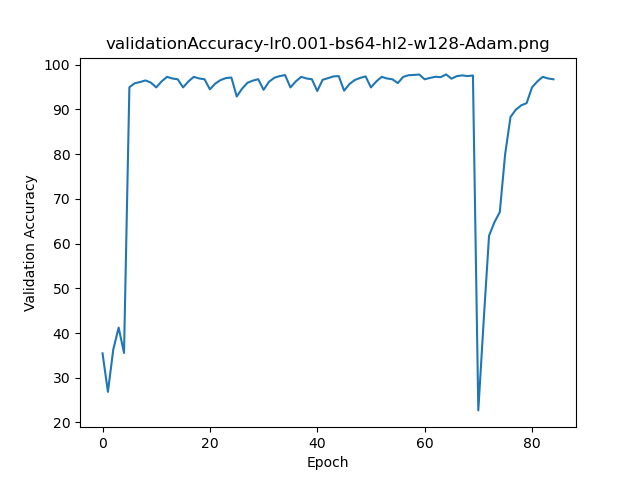
\includegraphics[width=\linewidth]{testsResults/validationAccuracy/def.png}
        \caption{Default settings + learning rate = 0.1}
        \endminipage
    \end{figure}

\subsubsection{Mini-Batch size}

    \begin{figure}[H]
        \minipage{0.5\textwidth}
        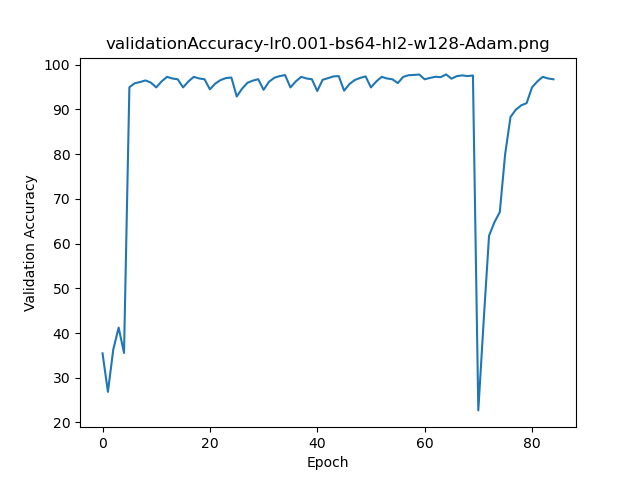
\includegraphics[width=\linewidth]{testsResults/validationAccuracy/def.png}
        \caption{Default settings + batching size = 64}
        \endminipage\hfill
        \minipage{0.5\textwidth}
        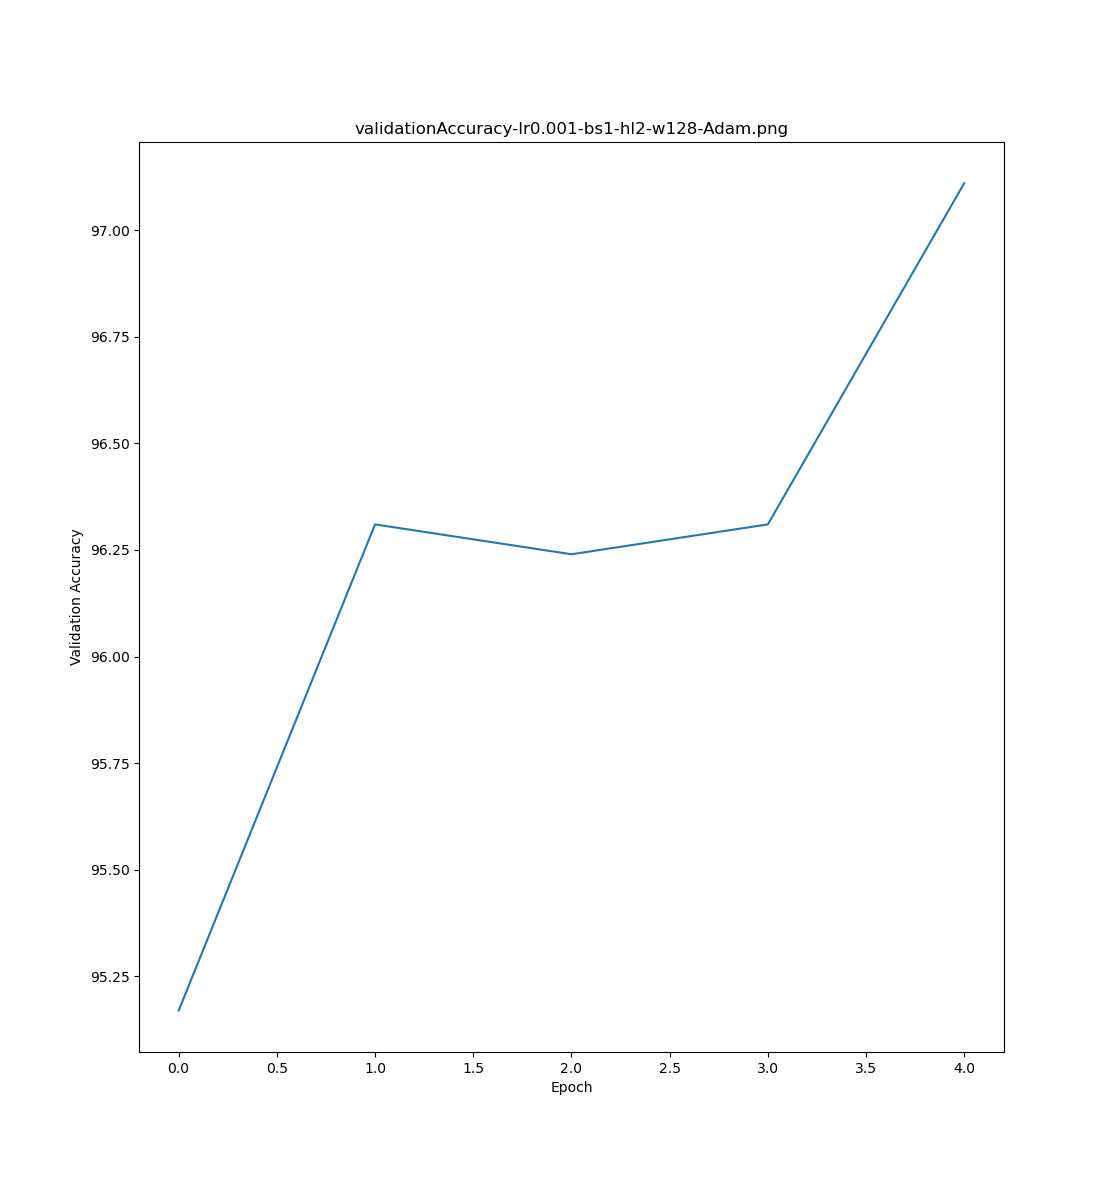
\includegraphics[width=\linewidth]{testsResults/validationAccuracy/validationAccuracy1batch.png}
        \caption{Default settings + batching size = 1}
        \endminipage
    \end{figure}
        \begin{figure}[H]
        \minipage{0.5\textwidth}%
        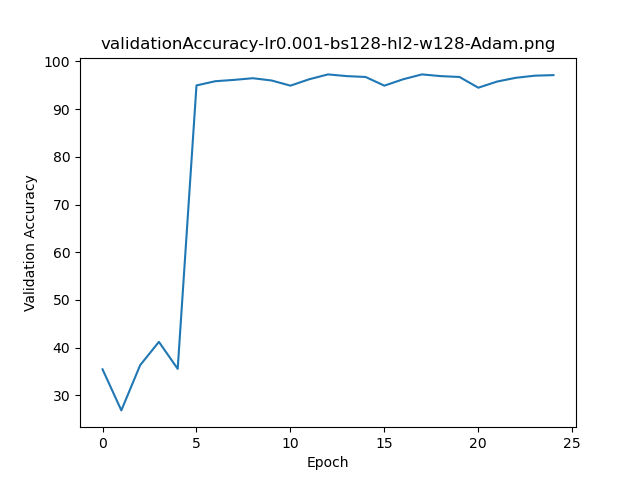
\includegraphics[width=\linewidth]{testsResults/validationAccuracy/validationAccuracy-lr0.001-bs128-hl2-w128-Adam.png}
        \caption{Default settings + batching size = 128}
        \endminipage
        \minipage{0.5\textwidth}%
        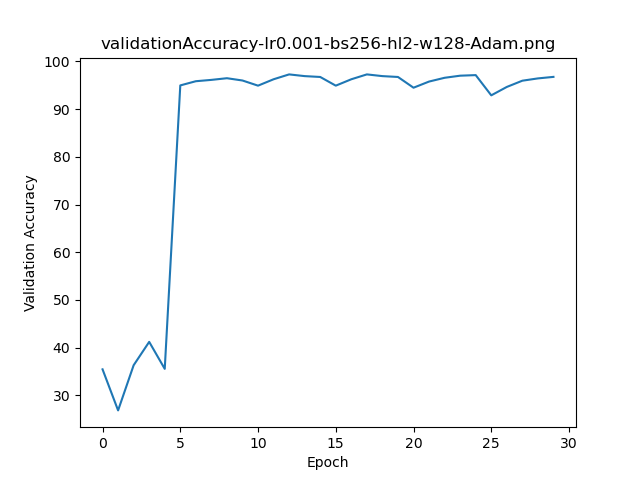
\includegraphics[width=\linewidth]{testsResults/validationAccuracy/validationAccuracy-lr0.001-bs256-hl2-w128-Adam.png}
        \caption{Default settings + batching size = 256}
        \endminipage
    \end{figure}

\subsubsection{Number of Hidden Layers}

    \begin{figure}[H]
        \minipage{0.5\textwidth}
        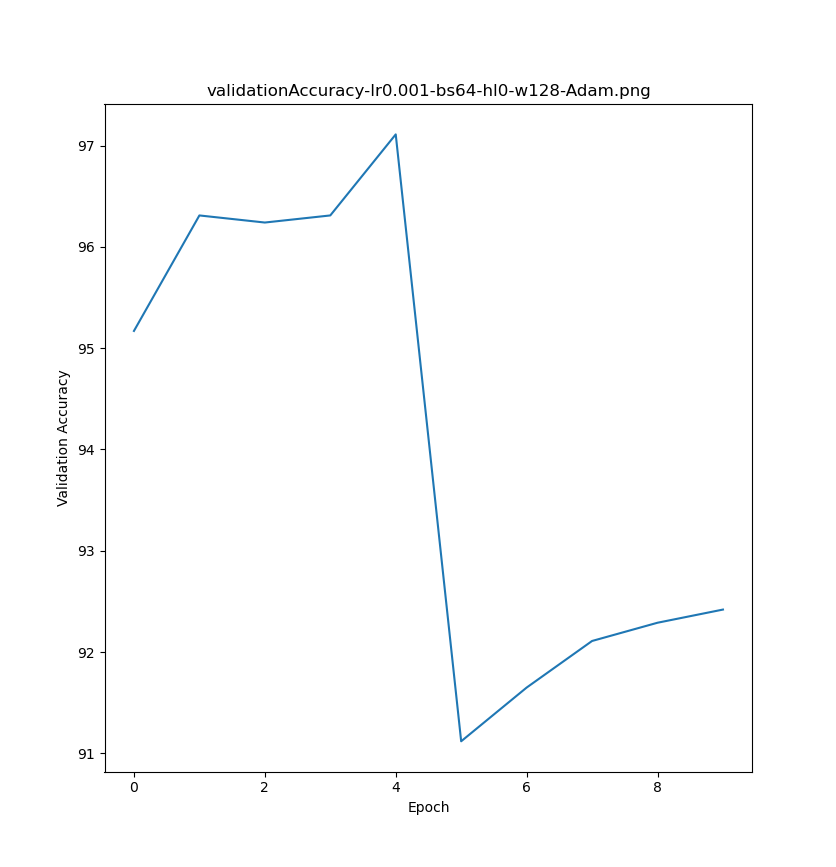
\includegraphics[width=\linewidth]{testsResults/validationAccuracy/validationAccuracyhl0.png}
        \caption{Default settings + hidden layers = 0}
        \endminipage\hfill
        \minipage{0.5\textwidth}
        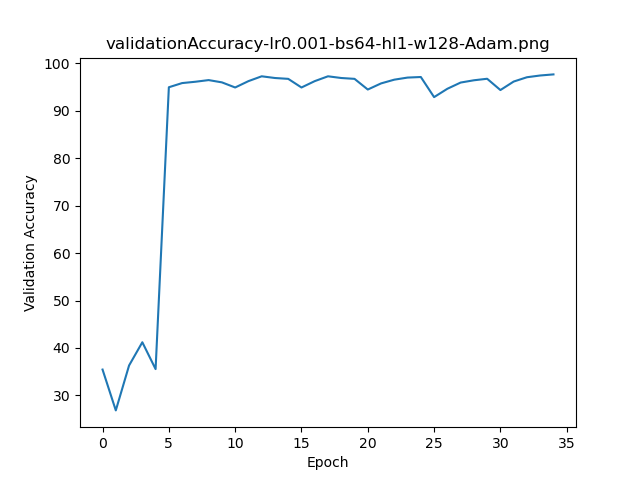
\includegraphics[width=\linewidth]{testsResults/validationAccuracy/validationAccuracy-lr0.001-bs64-hl1-w128-Adam.png}
        \caption{Default settings + hidden layers = 1}
        \endminipage
    \end{figure}
        \begin{figure}[H]
        \minipage{0.5\textwidth}%
        \includegraphics[width=\linewidth]{testsResults/validationAccuracy/def.png}
        \caption{Default settings + hidden layers = 2}
        \endminipage
        \minipage{0.5\textwidth}%
        \includegraphics[width=\linewidth]{testsResults/validationAccuracy/validationAccuracy-lr0.001-bs64-hl3-w128-Adam.png}
        \caption{Default settings + hidden layers = 3}
        \endminipage
    \end{figure}
    \newpage
\subsubsection{Width}

    \begin{figure}[H]
        \minipage{0.5\textwidth}
        \includegraphics[width=\linewidth]{testsResults/validationAccuracy/def.png}
        \caption{Default settings + width = 128}
        \endminipage\hfill
        \minipage{0.5\textwidth}
        \includegraphics[width=\linewidth]{testsResults/validationAccuracy/validationAccuracy-lr0.001-bs64-hl2-w64-Adam.png}
        \caption{Default settings + width = 64}
        \endminipage
    \end{figure}
        \begin{figure}[H]
        \minipage{0.5\textwidth}%
        \includegraphics[width=\linewidth]{testsResults/validationAccuracy/validationAccuracy-lr0.001-bs64-hl2-w256-Adam.png}
        \caption{Default settings + width = 256}
        \endminipage
        \minipage{0.5\textwidth}%
        \includegraphics[width=\linewidth]{testsResults/validationAccuracy/validationAccuracy-lr0.001-bs64-hl2-w512-Adam.png}
        \caption{Default settings + width = 512}
        \endminipage
    \end{figure}
    \begin{figure}[H]
        \minipage{0.5\textwidth}%
        \includegraphics[width=\linewidth]{testsResults/validationAccuracy/validationAccuracy-lr0.001-bs64-hl2-w1024-Adam.png}
        \caption{Default settings + width = 1024}
        \endminipage
    \end{figure}

\subsubsection{Optimizer Type}

    \begin{figure}[H]
        \minipage{0.5\textwidth}
        \includegraphics[width=\linewidth]{testsResults/validationAccuracy/def.png}
        \caption{Default settings + Adam optimizer}
        \endminipage\hfill
        \minipage{0.5\textwidth}
        \includegraphics[width=\linewidth]{testsResults/validationAccuracy/validationAccuracy-lr0.001-bs64-hl2-w128-SGD.png}
        \caption{Default settings + learning rate = 0.01}
        \endminipage
    \end{figure}
        \begin{figure}[H]
        \minipage{0.5\textwidth}%
        \includegraphics[width=\linewidth]{testsResults/validationAccuracy/validationAccuracy-lr0.001-bs64-hl2-w128-SGD_Momentum.png}
        \caption{Default settings + SGD\_Momentum optimizer}
        \endminipage
    \end{figure}


\end{document}
